\documentclass[11pt]{article}

\usepackage[margin=1in]{geometry}
\usepackage[utf8]{inputenc}
\usepackage[T1]{fontenc}
\usepackage{amsmath, amssymb}
\usepackage{graphicx}
\usepackage{booktabs}
\usepackage{enumitem}
\usepackage[hidelinks]{hyperref}
\usepackage[numbers]{natbib}
\usepackage{xcolor}
% Dark mode: comment out the next line for normal black-on-white
% \AtBeginDocument{\pagecolor{black}\color{white}}

% ---------------------------------------------------------------------------
% Paper details -- fill these in for each review
% ---------------------------------------------------------------------------
\newcommand{\papertitle}{STONE: A Spatio-temporal OOD Learning Framework Kills Both Spatial and Temporal Shifts}
\newcommand{\paperauthors}{Wang and Ma et al.}
\newcommand{\papervenue}{Proceedings of the 30th ACM SIGKDD}
\newcommand{\paperlink}{\url{https://doi.org/10.1145/3637528.3671680}}
\newcommand{\paperkey}{author2024example} % BibTeX key in references.bib
\newcommand{\reviewdate}{\today}

\title{Review: \papertitle}
\author{}
\date{\reviewdate}

\begin{document}

\maketitle

\begin{tabular}{@{}ll@{}}
  \textbf{Authors:} & \paperauthors \\
  \textbf{Published:} & \papervenue \\
  \textbf{Link:} & \paperlink \\
  \textbf{Citation:} & \cite{wang_stone_2024} \\
\end{tabular}

\section{Abstract}
Traffic prediction is a crucial task in the Intelligent Transportation System (ITS), receiving significant attention from both industry and academia. Numerous spatio-temporal graph convolutional networks have emerged for traffic prediction and achieved remarkable success. However, these models have limitations in terms of generalization and scalability when dealing with Out-of-Distribution (OOD) graph data with both structural and temporal shifts. To tackle the challenges of spatio-temporal shift, we propose a framework called STONE by learning invariable node dependencies, which achieve stable performance in variable environments. STONE initially employs gated-transformers to extract spatial and temporal semantic graphs. These two kinds of graphs represent spatial and temporal dependencies, respectively. Then we design three techniques to address spatio-temporal shifts. Firstly, we introduce a Fréchet embedding method that is insensitive to structural shifts, and this embedding space can integrate loose position dependencies of nodes within the graph. Secondly, we propose a graph intervention mechanism to generate multiple variant environments by perturbing two kinds of semantic graphs without any data augmentations, and STONE can explore invariant node representation from environments. Finally, we further introduce an explore-toextrapolate risk objective to enhance the variety of generated environments. We conduct experiments on multiple traffic datasets, and the results demonstrate that our proposed model exhibits competitive performance in terms of generalization and scalability.

\subsection{Keywords}
Spatio-temporal data mining, Out-of-distribution generalization, Traffic prediction, Causal graph learning

\section{Introduction}
\begin{itemize}
  \item GPS-enabled mobile data is a valuable asset in realm of urban computing
  \item Current traffic flow prediction uses data in graph-structured data in spatio-temporal graphs (STG)
  \item STG convolutional networks used to make spatio-temporal features and make predictions
  \item For graph \textbf{G} and training data \textbf{X} in the environment $e:\{\textbf{X}, \textbf{G}\}$, STG prediction learnings function $\mathcal{F}$ that predicts target $y$ given input $x$:
  \[
    \underset{\mathcal{F}}{\text{min}} \mathbb{E}_{(x, y)\sim P(x, y\vert e)}[\mathcal{L}(\mathcal{F}(\textbf{x}),y)\vert e]
  \]
  \item Models are succesful bur heavily depend on IID assumption, not true in real world where STG may change over time, posing issues with OOD scenarios
  \item Recent work in OOD spatio-temporal learning focusing on temporal shift but not spatial
\end{itemize}

\begin{figure}[h]
\centering
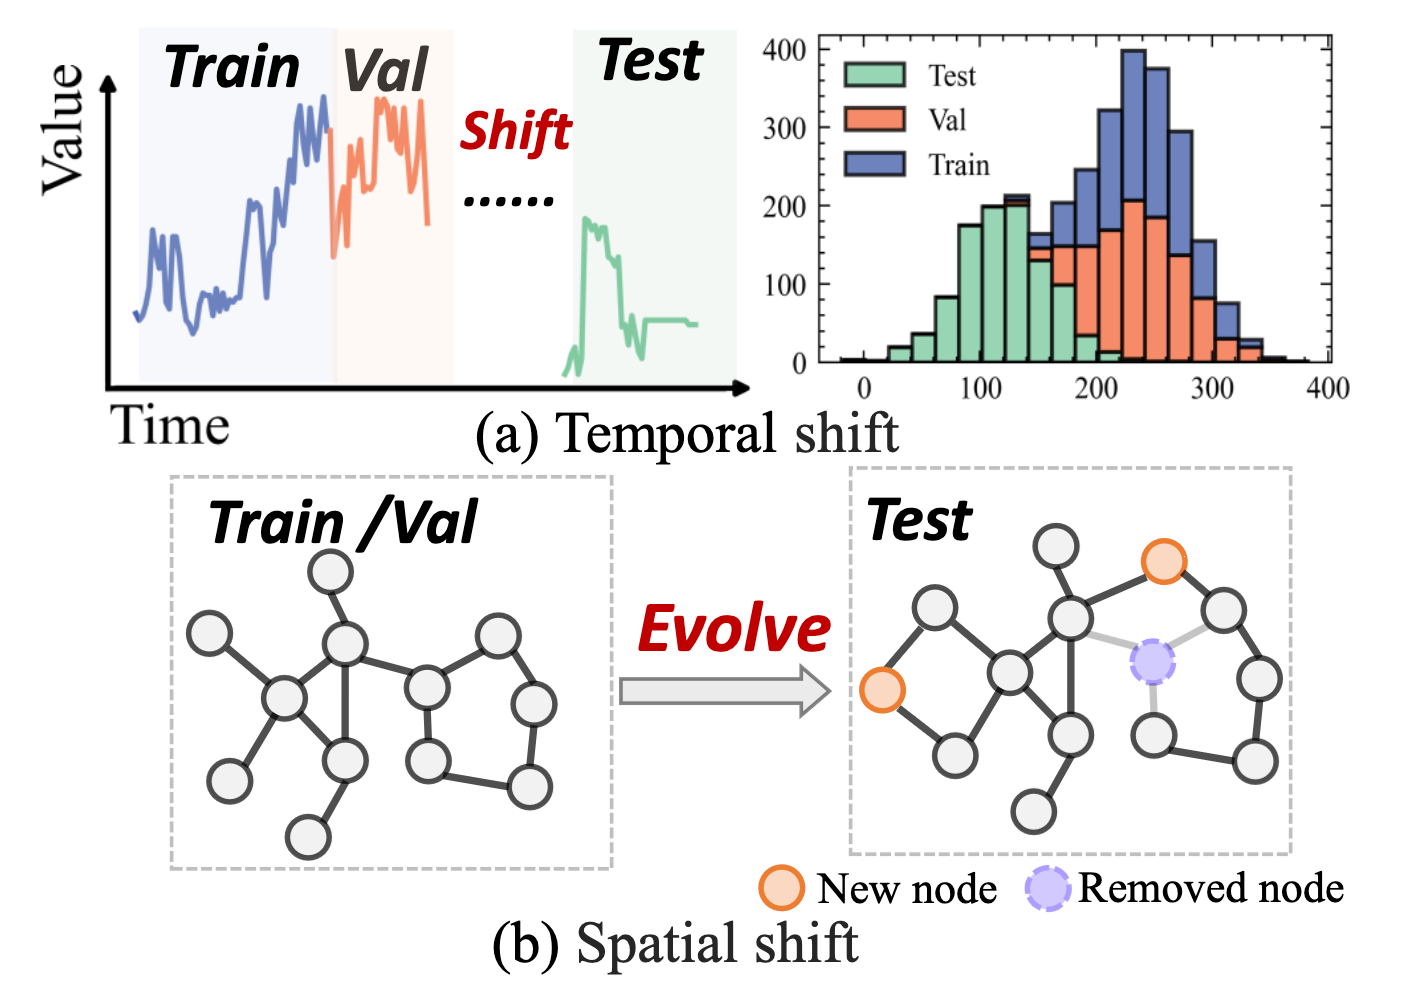
\includegraphics[width=0.8\textwidth]{figs/fig1.png}
\label{fig:fig1}
\caption{Temporal and spatial shift}
\end{figure}


\begin{enumerate}[label=(\alph*)]
  \item Temporal shift refers to change in temporal data distribution, $P(\textbf{X}_{te}) \neq P(\textbf{X}_{tr})$
  \item Spatial shift reffers to the evolution of underlying graph structure. Example is new or removed traffic sensor nodes in network
\end{enumerate}

\noindent Formally 


\bibliographystyle{plainnat}
\bibliography{references}

\end{document}
